\label{sec:hadhad_multijet}

Multi-jet production represents a relevant source of background in the
\hadhad signal region, with both \tauhadvis candidates originating
from the misidentification of quark- or gluon-initiated jets. It
represents the second largest background with \faketauhadvis in the
\hadhad SR after the dominant \ttbarFakes contribution.

The multi-jet background is estimated using the fake factor method
which is a data-driven method for background estimation. The method is
applicable in cases where two observables\footnote{For the fake factor
  method one observable is related to identification or isolation
  criteria of reconstructed physics objects, distinuishing it from the
  more general ABCD method.} exist that are statistically independent
for the background process, while also being strong discriminators
between the background process of interest and more signal-like
events. Four disjoint regions can be defined, three
background-enriched CRs and a SR, by applying selections on both
observables. The independence assumption allows to relate the observed
number of background events in the three CRs with the background
expectation in the SR, yielding data-driven estimate of the background
in the SR.

\begin{figure}[htbp]
  \centering

  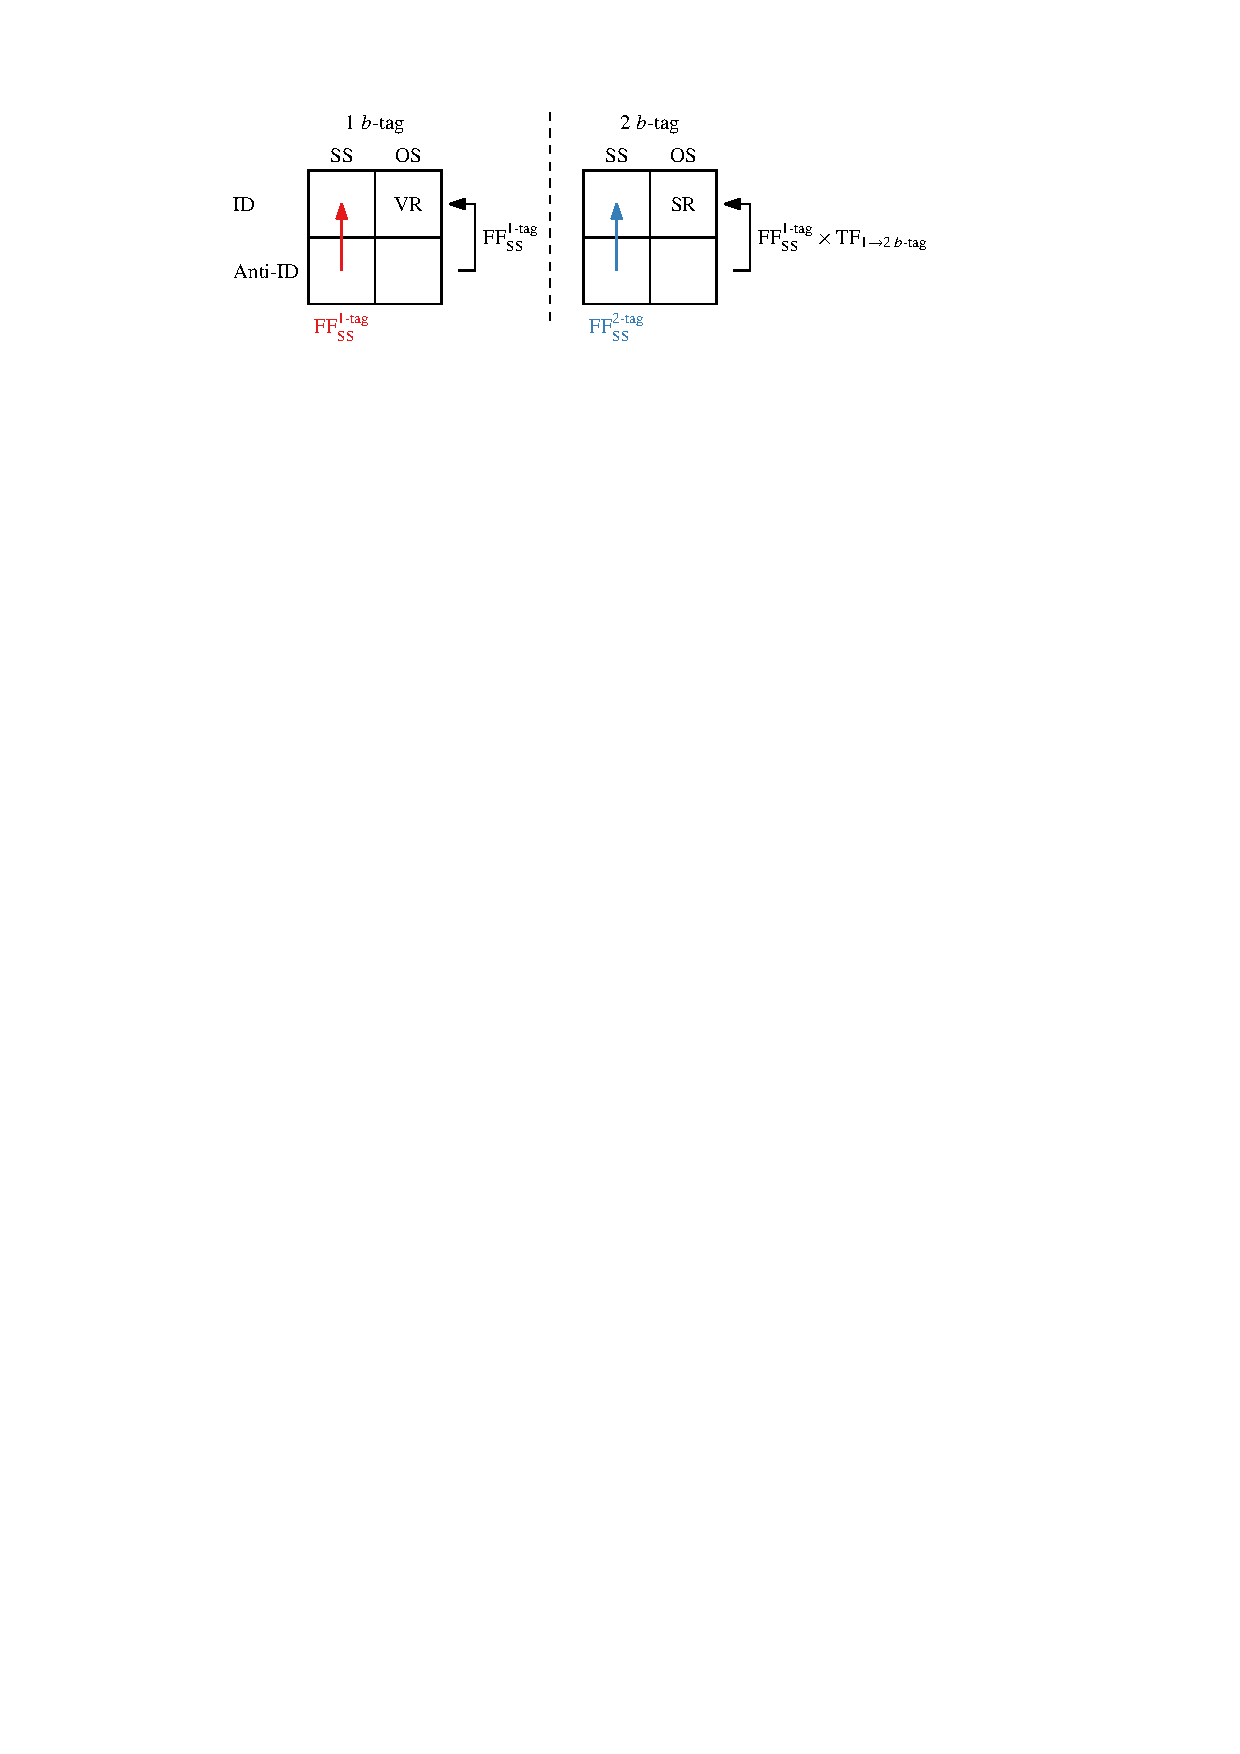
\includegraphics[scale=1]{fakefactors/regions}

  \caption{Region definitions}
  \label{fig:fakefactor_regions}
\end{figure}

Checked in 1-tag OS. Does agreement in 1-tag OS confirm that charge
and ID are independent?

\begin{itemize}
\item General idea of FFs (ABCD-like method): Derived under the
  assumption that the the probability of multi-jet events to pass into
  either ID or Anti-ID region is independent of the charge.

\item Definition of regions (OS, SS / ID, Anti-ID) Maybe a figure?

\item Anti-ID region definition: Limitation due to ATLAS data
  reduction in derivations (at least one loose tau -- prevents doing
  AA; minimum RNN > 0.01 -- prevents full Anti-ID)

\item Meausrement region: 1-tag (2-tag too little multi-jet purity due
  to large contamination of \faketauhadvis from \ttbar, also low statistical precision)

\end{itemize}












Events where one or more \tauhadvis is faked by jets originating from quarks or
gluons are estimated from dedicated control regions. Three fake enriched regions
are defined by requiring:
\begin{enumerate}
\item Same sign electric charge \tauhadvis (SS)
\item Exactly one \tauhadvis failing \textit{loose} identification but passing a
  lower cut of 0.01 on the RNN Tau-ID score (Anti-ID)
\item Both
\end{enumerate}
The four regions are henceforth called: OS ID, OS Anti-ID, SS ID, and SS
Anti-ID.

The fake factor (FF) measures the ratio of events with fake \tauhadvis in ID and
Anti-ID region:
\begin{align*}
  \FF = \frac{N\left( \text{fake} \, \tauhadvis, \text{ID} \right)}{N\left( \text{fake} \, \tauhadvis, \text{Anti-ID} \right)}
\end{align*}
The probability of a jet faking a \tauhadvis depends strongly on \tauhadvis \pT
and decay mode. Therefore, the fake factor is frequently parametrised in these
quantities. It is also affected by the \tauhadvis identification already applied
in the high-level \tauhadvis-triggers which also needs to be taken into account.

The fake factors are measured in the fake enriched SS-region by subtracting
non-fake-\tauhadvis background using their estimates from simulation:
\begin{align*}
  \FF_\text{SS} = \frac{N(\text{SS}, \text{ID}) - N_\text{non-fake}(\text{SS}, \text{ID})}{N(\text{SS}, \text{Anti-ID}) - N_\text{non-fake}(\text{SS}, \text{Anti-ID})}
\end{align*}
where $N$ is the total yield and $N_\text{non-fake}$ the yield of
non-fake-\tauhadvis backgrounds in the corresponding region.

To obtain the fake \tauhadvis estimate in the OS ID-region, the assumption is
made that the fake factors are independent of the reconstructed charge of the
fake \tauhadvis candidates. Therefore, the SS fake factors $\FF_\text{SS}$ are
applied to events in the OS Anti-ID region after subtracting any
non-fake-\tauhadvis contributions.
\begin{align*}
  N(\text{fake}, \text{OS ID}) = \FF_\text{SS} \times \left[ N(\text{OS}, \text{Anti-ID}) - N_\text{non-fake}(\text{OS}, \text{Anti-ID}) \right]
\end{align*}
Systematic uncertainties are assigned to
cover possible difference betwen OS and SS fake factors, varying the
subtraction in the OS Anti-ID region. Moreover, the fake factors are
independently varied by their statistical uncertainty.

Due to the limited acceptance of fake \tauhadvis in the 2 \btag region, the 1
\btag region is used to calculate the fake factors instead. The 1 \btag fake
factors are applied to the 2 \btag OS Anti-ID region and an additional 1 to 2
\btag transfer factor is applied.

The binning of the fake factors is dependent on the trigger that selected the
event. For STT events the fake factor is binned in whether the anti-\tauhadvis
is leading or subleading in \pT, and the decay mode of the \tauhadvis
($N_\text{track}$). Due to low statistics in the STT category the fake factors
are inclusive in \tauhadvis \pT. The \tauhadvis identification at the HLT is
only applied to one of the two \tauhadvis candidates affecting the probability
of jets faking \tauhadvis, motivating the binning in whether the leading /
subleading \tauhadvis fails the identification.

For DTT events, HLT \tauhadvis identification is applied to both \tauhadvis
candidates. Therefore, the fake factors do not need to distinguish between cases
where the leading and subleading \tauhadvis fails the loose identification. The
fake factors for DTT events are parametrised in the \pT and decay mode of the
the \tauhadvis candidate failing the identification requirement.

Moreover, all fake factors are binned by data-taking period (${\text{2015-2016},
  \text{2017}, \text{2018}}$) which takes into account the different triggers
being used to select events used for the analysis.

\todo[inline]{Could we use nOS to enhance statistics? Maybe flip the FF method
  so that we use events in SS ID to build the template instead of OS Anti-ID.}

\todo[inline]{Can we make the STT FF depend on the trigger-match instead of
  the leading / subleading binning?}


%%% Local Variables:
%%% mode: latex
%%% TeX-master: "../../phd_thesis"
%%% End:
